\documentclass[border=3pt]{standalone}
% Preâmbulo compartilhado pelos diagramas TikZ da aula 7 (Filtros Não Paramétricos)
\usepackage[T1]{fontenc}
\usepackage[utf8]{inputenc}
\usepackage{lmodern}
\usepackage{amsmath}
\usepackage{xcolor}
\usepackage{tikz}
\usetikzlibrary{arrows.meta,angles,quotes,decorations.pathmorphing,calc,
                positioning,shapes.geometric,shapes.misc,backgrounds,fit,
                math}

% Paleta (mesma dos SVGs originais)
\definecolor{dblue}{HTML}{2A5B8C}
\definecolor{dorange}{HTML}{B3541E}
\definecolor{dgreen}{HTML}{4A7C59}
\definecolor{dred}{HTML}{9C4B4B}
\definecolor{dcream}{HTML}{F4F1EA}
\definecolor{dshade}{HTML}{DDD7C9}

% Função gaussiana (não normalizada por padrão de escala visual)
\pgfmathdeclarefunction{gauss}{3}{%
  \pgfmathparse{1/(#3*sqrt(2*pi))*exp(-((#1-#2)^2)/(2*#3^2))}%
}

% Estilos comuns (prefixo d... para não colidir com chaves internas do pgf)
\tikzset{
  >={Stealth[length=2mm]},
  dguide/.style={gray!55, dashed, line width=0.4pt},
  daxis/.style={gray!60, line width=0.7pt, ->},
  dbody/.style={fill=black!3, draw=black!80, line width=1pt},
  dacc/.style={draw=dblue, line width=1pt},
  dlbl/.style={black!55, font=\small},
  dsub/.style={black!45, font=\footnotesize},
  dstate/.style={circle, draw=black!80, fill=dcream, line width=1pt,
                 minimum size=17mm, font=\large, inner sep=1pt},
  dobs/.style={circle, draw=black!80, fill=dshade, line width=1pt,
               minimum size=14mm, font=\large, inner sep=1pt},
  dbox/.style={rounded corners=2pt, draw=black!80, fill=dcream, line width=1pt,
               align=center, inner sep=6pt},
  dop/.style={circle, draw=black!80, fill=white, line width=1pt,
              minimum size=6mm, inner sep=0pt, font=\small},
  dtrans/.style={->, dblue, line width=1pt},
  dmeas/.style={->, dorange, line width=1pt},
  dcurve/.style={line width=1pt, dblue},
  dcurveb/.style={line width=1.4pt, dorange},
}

\begin{document}
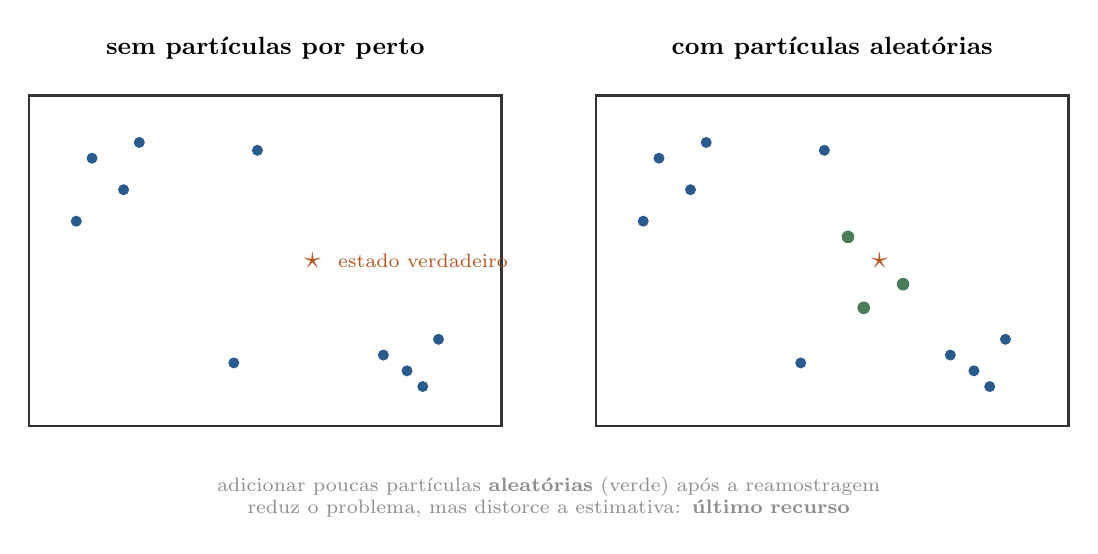
\begin{tikzpicture}[x=1cm,y=1cm]
  \newcommand{\espaco}{\draw[dbody, fill=white, line width=1pt] (0,0) rectangle (6,4.2);}
  \begin{scope}
    \espaco
    \foreach \x/\y in {0.8/3.4,1.2/3.0,0.6/2.6,1.4/3.6,4.8/0.7,5.2/1.1,4.5/0.9,5.0/0.5,2.6/0.8,2.9/3.5} { \fill[dblue] (\x,\y) circle (0.07); }
    \node[dorange, font=\large] at (3.6,2.1) {$\star$}; \node[dorange, font=\scriptsize, anchor=west] at (3.8,2.1) {estado verdadeiro};
    \node[font=\small\bfseries] at (3,4.8) {sem partículas por perto};
  \end{scope}
  \begin{scope}[shift={(7.2,0)}]
    \espaco
    \foreach \x/\y in {0.8/3.4,1.2/3.0,0.6/2.6,1.4/3.6,4.8/0.7,5.2/1.1,4.5/0.9,5.0/0.5,2.6/0.8,2.9/3.5} { \fill[dblue] (\x,\y) circle (0.07); }
    \foreach \x/\y in {3.2/2.4,3.9/1.8,3.4/1.5} { \fill[dgreen] (\x,\y) circle (0.08); }
    \node[dorange, font=\large] at (3.6,2.1) {$\star$};
    \node[font=\small\bfseries] at (3,4.8) {com partículas aleatórias};
  \end{scope}
  \node[dsub, font=\scriptsize, align=center, text width=13cm] at (6.6,-0.9) {adicionar poucas partículas \textbf{aleatórias} (verde) após a reamostragem reduz o problema, mas distorce a estimativa: \textbf{último recurso}};
\end{tikzpicture}
\end{document}
